%% Introduction 
%%	What is this chapter all about? 
%%	What sub-problem or issue is this chapter addressing? 
%%	How does this chapter fit within the overall “story” of the thesis? 
%%The Meat
%%	Rigorous approach to sub-problem, or detailed explanation of issue
%%	Assumptions underlying sub-problem, or complete description of issue
%%	Validation: System design, theory, implementation, graphs, references, …. 
%%Summary
%%	Repeat the highlights of the chapter
%%	Transition sentence that acts as a “teaser” for the next chapter, and how the next chapter fits with the current one


\section{Introduction}

\todo{Review comment: Start with something like ``This chapter provides...'' and give high level view. [DONE]}

\added{The previous chapter presented an overview of the newly proposed system called ``\mysystemname'' and its architecture. This chapter provides details of its first module, called Model Defeaturing, i.e. the algorithms proposed for defeaturing sheet metal feature based CAD model.}

Defeaturing is one of the most popular approaches of simplifying CAD models for CAE analysis. 
\added{CAD models contain various details (or features in case the CAD model is feature based) which are introduced due to requirements of various downstream applications such as CAM, Visualization, etc. Such detailed models are often not needed for CAE, especially for quicker validations at the early stages of design.} Defeaturing is the process of removing irrelevant details or features in the context of application to generate the simplified model, called ``gross shape''\deleted{(Definition \ref{def:grossshape})}. It is the principal shape that ``represents'' the input shape, but with lesser features. In CAE analysis, the finite element mesh generated on the gross shape that is obtained by defeaturing has far lesser number of nodes compared to the original input CAD model. Lesser number of nodes means lesser number of degrees of freedoms (DoFs) for solving the CAE equations, thus lesser computations and quicker analysis results. 

\todo{Review comment: Make this (``Defeaturing is primarily...'') earlier. [BROUGHT HERE]}
\todo{Review comment: Just mention that defeaturing typically helps in significantly reducing DoFs in CAE analysis.[DONE]}

%%\bigskip

	\begin{figure} [!h]
		\centering
		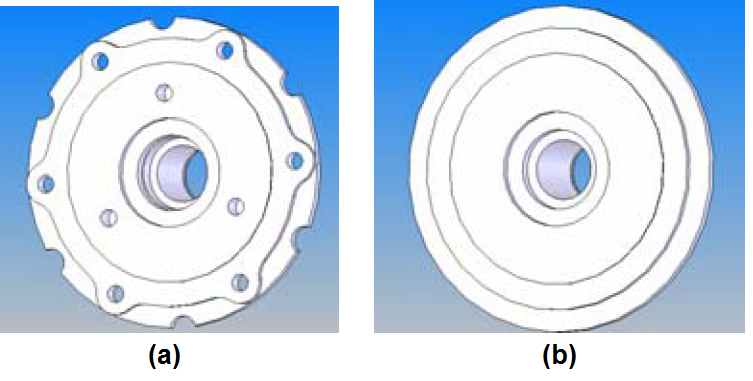
\includegraphics[width=0.7\linewidth]{..//Common/images/GopalDefeat.png}
		\caption{Gross Shape of Rotor Brake (Source: Gopalkrishnan~\cite{GopalakrishnanSuresh2007})}
		\label{fig:defeaturing:gopaldefeat}
	\end{figure}
	
%%\bigskip

\replaced{Figure  \ref{fig:defeaturing:gopaldefeat}a shows a CAD model of a Rotor Brake part. It has about 50 distinct features and all of them are not relevant for the thermal analysis. After defeaturing, i.e. after removing small holes, depressions, cutouts, etc. the output gross shape is shown in Figure  \ref{fig:defeaturing:gopaldefeat}b.  Gopalakrishnan~\cite{GopalakrishnanSuresh2007} reported that, in this particular example, DoFs got reduced from 150,000 to 25,000 after defeaturing, thereby speeding up the computation significantly.}{Gopalkrishnan \cite{GopalakrishnanSuresh2007} showed that (Figure \ref{fig:defeaturing:gopaldefeat}) in case of rotor brake model, it has about 50 distinct features and all of them are not relevant for thermal analysis. After computing the ``gross shape'', i.e. removing the irrelevant features, DoFs in CAE analysis got reduced from 150,000 to 25,000, thereby speeding the computation significantly.}

Apart from CAE, gross shapes are also used in shape matching \& retrieval, faster visualizations, hiding proprietary details, quicker transmissions across the networks, etc. Reason being, it is far more efficient to work on the gross shape (which retains the important shape characteristics) than the detailed input CAD model. Thus, due to these advantages, defeaturing usage is found in a wide variety of applications.

The core decision in any defeaturing approach is the criterion of `irrelevance' of a detail or feature in the context of application, which is CAE in this case. For example, for structural CAE analysis, following could be the criteria:

\begin{itemize}[noitemsep,topsep=2pt,parsep=2pt,partopsep=2pt]
\item Remove small fillets \& chamfers. Results of the analysis will show increase in the stresses in the gross shape compared to the original input model. So the results will be conservative and safer for further part design steps.
%\item Remove  Holes will result in an analysis showing lower stresses than the actual case which must somehow be taken into account. \deleted{so that the final design will have sufficient strength.}
\item Do not remove features in the load path and near Boundary Conditions. They are critical to the results and are not to be removed even if they are eligible for removal due to smaller sizes.
\end{itemize}

The present research work takes sheet metal feature-based CAD model as input for computing midsurface. Hypothesis~\ref{hyp:Simplification} which says that the gross shape enhances definitiveness of getting a quality midsurface, is tested in this chapter. Following sections present systematic study of sheet metal feature characteristics to decide the eligibility of some of them for removal.
	
%The research presented here does not take any application-context-specific input data, so it is agnostic to it now, but later, with those inputs available, the method can be tailored to incorporate application-context specific rules as well.
%\footnote{Terms `Defeaturing' and `Simplification', both are used synonymously in this work, unless specified otherwise} 